\documentclass{beamer}
\usepackage{graphicx}
\usepackage{caption}
\usepackage{hyperref}
\usepackage{array}

\title{Containerization in the Linux Kernel}
\author{Kilian Calefice (796461)}
\institute{Linux Internals}
\date{09.09.2024}

\begin{document}

\frame{\titlepage}

\begin{frame}
  \frametitle{Gliederung}
  \begin{itemize}
    \item Einführung
    \item Relevante Features des Kernels
    \item Funktionsweise
    \item Beispiel mit Docker
  \end{itemize}
\end{frame}

\begin{frame}
  \frametitle{Einführung}
  \begin{itemize}
    \item Container sind eine Abstraktion, um Prozesse isoliert auszuführen und 
      nutzen dabei verschiedene Kernel-Features
    \item Die meisten relevanten Kernel-Features wurden 2008 im Kernel eingeführt
  \end{itemize}
\end{frame}

\begin{frame}
  \frametitle{Virtual Machines vs. Container}
  \begin{figure}[h]
    \centering
    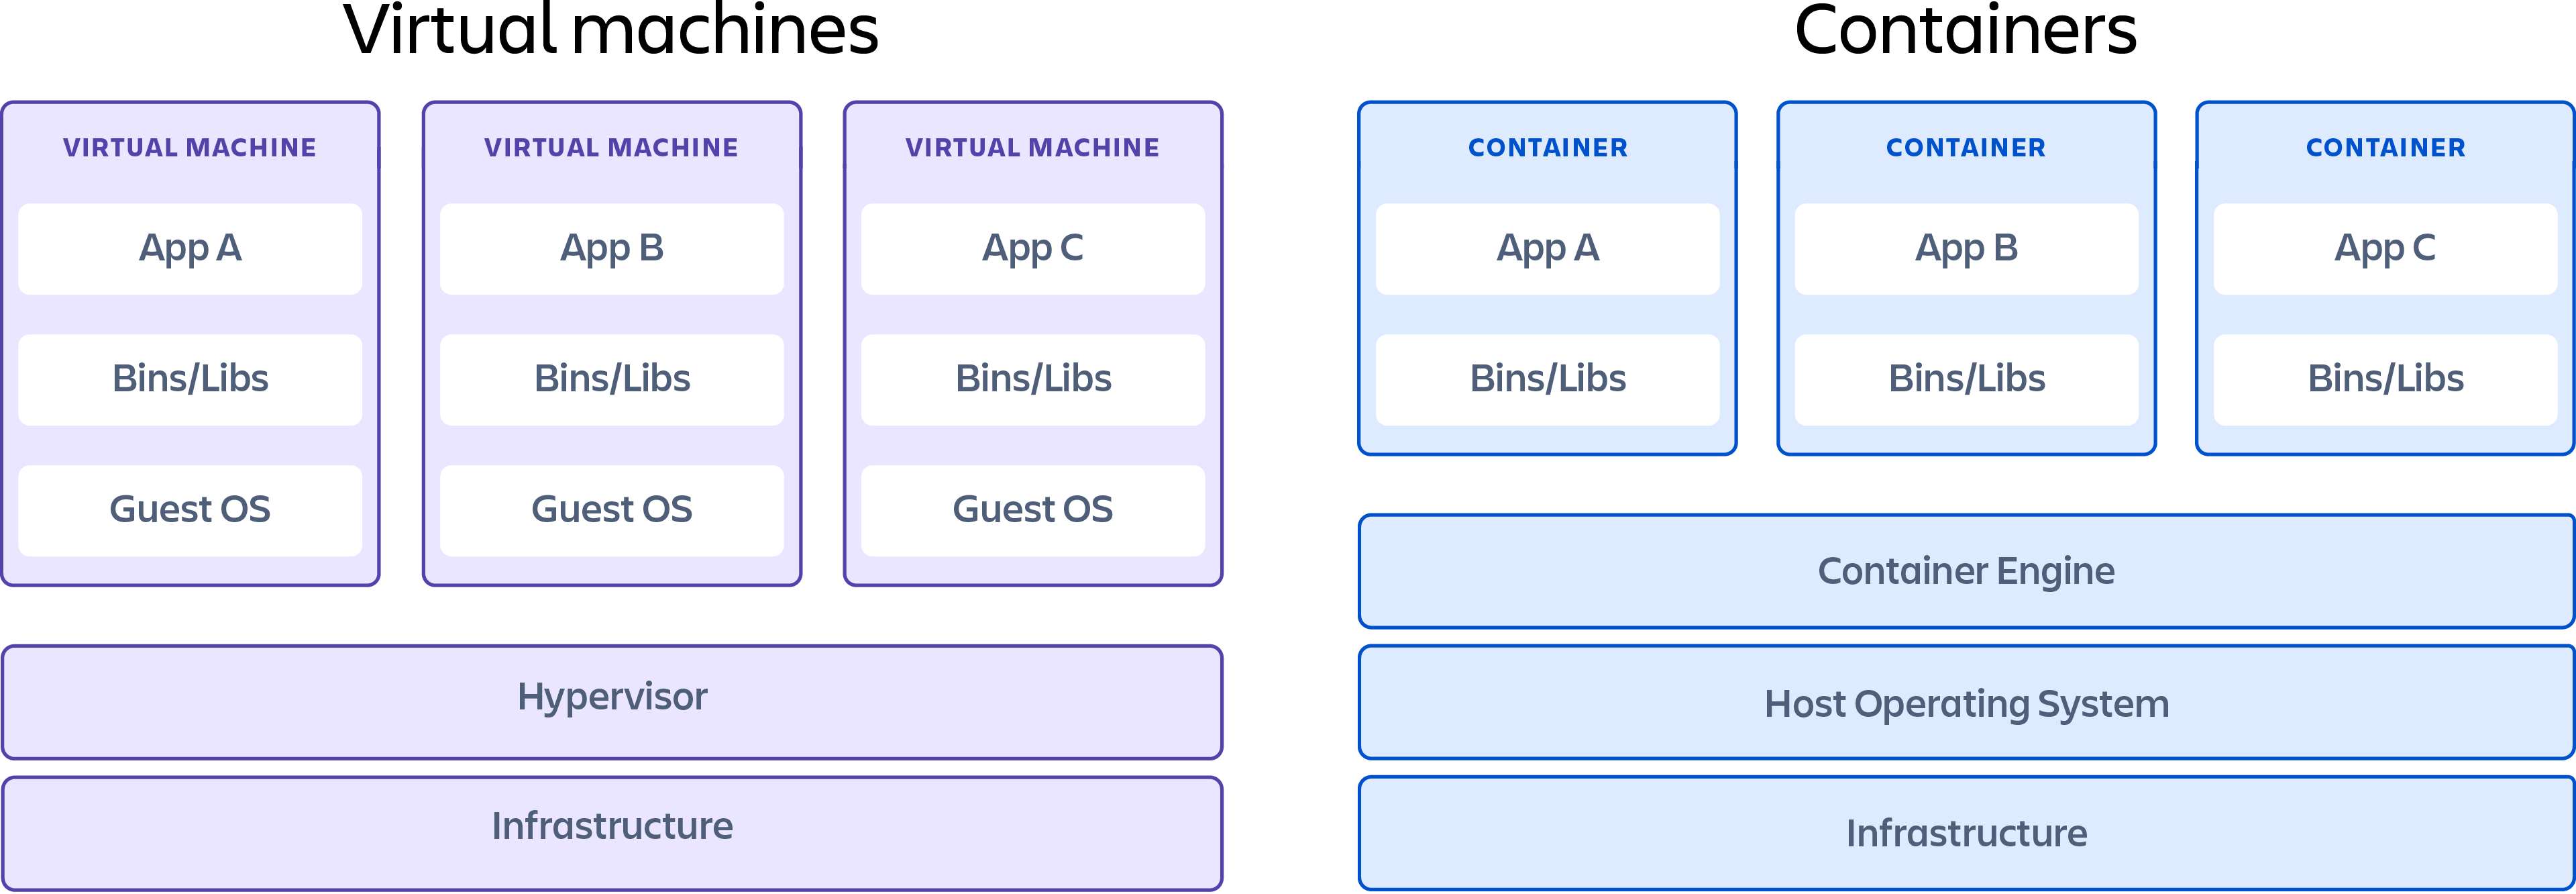
\includegraphics[width=\linewidth]{container-vs-vm.png}
    \caption*{{\tiny Abbildung 1}}
  \end{figure}
  \vfill
  {\tiny Abbildung 1: \href{https://wac-cdn.atlassian.com/dam/jcr:92adde69-f728-4cfc-8bab-ba391c25ae58/SWTM-2060_Diagram_Containers_VirtualMachines_v03.png}{https://wac-cdn.atlassian.com/dam/jcr:92adde69-f728-4cfc-8bab-ba391c25ae58/SWTM-2060\_Diagram\_Containers\_VirtualMachines\_v03.png}}
\end{frame}

\begin{frame}
  \frametitle{Kernel-Features}
  \begin{enumerate}
    \item Control Groups 
    \item Namespaces
    \item Overlay Filesystem
    \item ...
  \end{enumerate}
\end{frame}

\begin{frame}
  \frametitle{Control Groups} 
  \begin{itemize}
    \item Controller / Subsystems überwachen die Resourcennutzung im Kernel und sorgen dafür, dass Limits 
      eingehalten werden
    \item Hierarchiche File-Struktur in \texttt{/sys/fs/cgroup}, um cgroups zu definieren
    \item Limits werden von den Eltern-cgroups an Kind-cgroups vererbt
    \item Child Prozesse treten automatisch der Cgroup des Elternprozesses bei
  \end{itemize}
\end{frame}

\begin{frame}
  \frametitle{Namespaces}
  \begin{itemize}
    \item Es gibt pid, net, mnt, ipc, uts, user und cgroup namespaces
    \item Sind dazu da Kernelresourcen zu isolieren
    \item Mit \texttt{unshare} kann man eine neue Namespace erzeugen
    \item Eine Namespace kann nur mit einem Prozess in ihr existieren
  \end{itemize}
\end{frame}

\begin{frame}
  \frametitle{Overlay Filesystem}
  \begin{itemize}
    \item Filesystem besteht aus directories die auch als Layers bezeichnet werden (\textbf{Lower Layer}, \textbf{Upper Layer})
    \item Copy on write: Files werden nicht in tieferen Layers modifiziert sondern in eine neue Layer kopiert und dort modifiziert
    \item Merged view: Wenn man eine File lesen will guckt der Kernel in der obersten Layer und geht jeweils tiefer wenn er sie in der Layer nicht findet
  \end{itemize}
\end{frame}

\begin{frame}
  \frametitle{Quellen}
  \begin{itemize}
    \item {\href{https://docs.redhat.com/en/documentation/red_hat_enterprise_linux_atomic_host/7/html/overview_of_containers_in_red_hat_systems/introduction_to_linux_containers#overview}{Red Hat - Introduction to Linux Container}}
    \item {\href{https://www.youtube.com/watch?v=x1npPrzyKfs&t=1431s&ab_channel=linuxfestnorthwest}{Linux Fest - Container Pirimitives}}
    \item {\href{https://daveiscoding.hashnode.dev/why-do-you-need-an-init-process-inside-your-docker-container-pid-1#heading-signals}{Init PID - Docker Container}}
    \item {\href{https://www.youtube.com/watch?v=sK5i-N34im8&t=1541s&ab_channel=Docker}{Docker Con - Cgroups, namepsaces and beyond}}
  \end{itemize}
\end{frame}

\end{document}
